\section{辐射度学}\label{sec:辐射度学}

\keyindex{辐射度学}{radiometry}{}提供了一系列描述光传播与反射的思想和数学工具。
它为贯穿本书剩余部分的渲染算法构建了推导的基础。
有趣的是,辐射度学不是用物理光学基本原理推导产生的,
而是基于穿过空间的粒子流来对光进行抽象并建立的。
因此,尽管辐射度学和\keyindex{麦克斯韦方程组}{Maxwell's equations}{}之间
已经建立了联系,为辐射度学提供了坚实的物理基础,
但像光的\keyindex{偏振}{polarization}{}
\sidenote{译者注:指横波能够朝着不同方向振荡的性质。}
那样的效应并不符合该框架。

\keyindex{辐射转移}{radiative transfer}{}是关于辐射能量转移现象的研究。
它基于辐射度量原则并在\keyindex{几何光学}{geometrical optics}{}
\sidenote{译者注:原文写作geometric optics。}层面上操作,
其中光的宏观性质足以描述光如何与比其波长大得多的物体相交。
与光的\keyindex{波动光学}{wave optics}{}模型中的现象结合并不罕见,
但这些结果需要用辐射转移的基本抽象语言来表达。
(\citet{PREISENDORFER19653}已经将辐射转移理论与
麦克斯韦描述电磁场的经典方程组联系起来。
他的框架既论证了它们的等价性又使得把一个世界观的结果应用到另一个世界观更容易了。
\citet{Fante:81}在该领域做了更多最近的工作。)

用这种方法就能描述光和与其波长大小接近的物体相交,
进而对\keyindex{色散}{dispersion}{}\sidenote{译者注:经典的棱镜色散实验。}
\begin{marginfigure}
    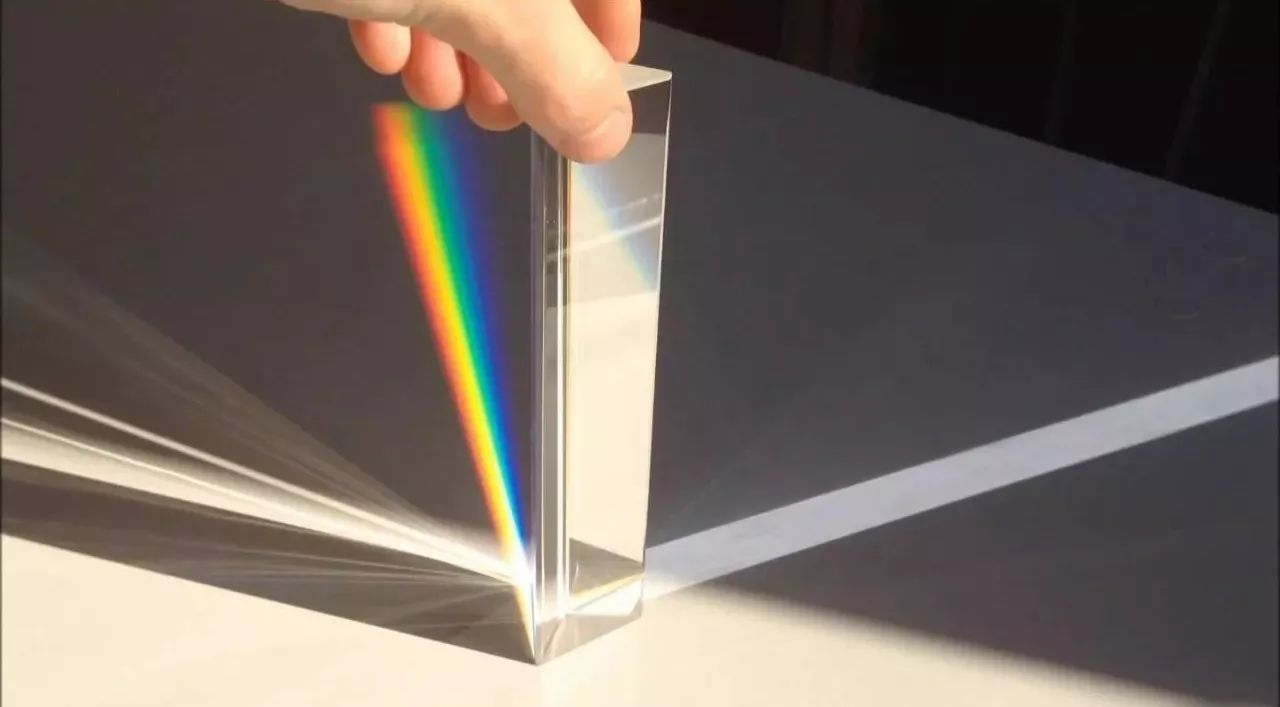
\includegraphics[width=\linewidth]{chap05/dispersion.jpg}
\end{marginfigure}
和\keyindex{干涉}{interference}{}\sidenote{译者注:经典的双缝干涉实验。}
\begin{marginfigure}
    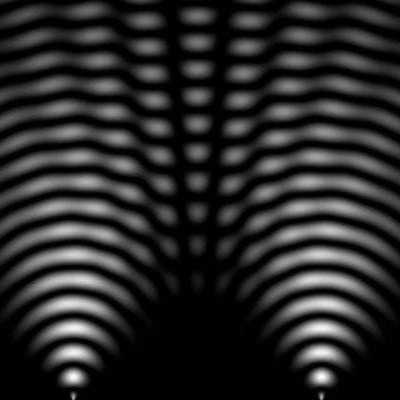
\includegraphics[width=\linewidth]{chap05/interference.jpg}
\end{marginfigure}
等效应建模。
在更精细的细节层面上,需要\keyindex{量子力学}{quantum mechanics}{}来描述光与原子的交互。
幸运的是,解决计算机图形学中的渲染问题不用直接模拟量子力学原理,
故避免了此类方法的复杂性。

在pbrt中,我们将假设几何光学是足够用来描述光与光散射的模型。
这导出了一些整个系统中隐含使用的关于光的行为的基本假设:
\begin{itemize}
    \item \keyindex{线性关系}{linearity}{}:光学系统两个输入的共同效应总是等于每个输入各自效应之和。
    \item \keyindex{能量守恒}{conservation of energy}{}\sidenote{译者注:原文写作energy conservation。}:
          当光从表面或介质散射时,触发的散射不会比它开始时产生更多的能量。
    \item {\sffamily 无偏振}:我们将忽略电磁场的偏振;
          因此,光的唯一相关属性是它关于波长(或等价地,\keyindex{频率}{frequency}{})的分布。
    \item {\sffamily 无}\keyindex{荧光}{fluorescence}{}或\keyindex{磷光}{phosphorescence}{}:
          某一波长的光的行为完全独立于其他波长或时间的光的行为。
          像偏振那样,要包含这些效应并不难,但它们为系统增加的实用价值相对较低。
    \item \keyindex{稳态}{steady state}{}:假设环境中的光达到平衡,
          所以其辐射分布不随时间变化。在现实场景中这对于光几乎是一瞬间发生的,
          所以在实践中这没什么限制。注意磷光也违反了稳态假设。
\end{itemize}

采用几何光学模型最明显的损失是很难考虑\keyindex{衍射}{diffraction}{}和干涉效应。
如\citet[p. 24]{PREISENDORFER19653}所述,这是个很难解决的问题,
例如,当存在这些效应时两区域的总通量不一定等于每个区域各自接收的功率之和。

\subsection{基本量}\label{sub:基本量}
有四个辐射度量数量\sidenote{译者注:依据中国国家标准GB 3102.6-93,
    这些量的名称大都可以省略“射”字,例如“辐射出射度”也可以称作
    “辐射出度”“辐出射度”“辐出度”,以此类推。后续译文将视情况使用全称或简称。}
是渲染的核心:\keyindex{通量}{flux}{}、
\keyindex{辐射照度}{irradiance}{}/\keyindex{辐射出射度}{radiant exitance}{}、
\keyindex{强度}{intensity}{}和\keyindex{辐射亮度}{radiance}{}。
它们每个都可以从能量(单位为焦耳)依次对时间、面积和方向取极限推导出来
\sidenote{译者注:可参考译者补充的\refsub{辐射度量}。}。
所有这些辐射度量数量一般都依赖于波长。
对于本章的剩余部分,我们不再明确这一依赖关系,但记住这一性质是很重要的。

\subsubsection*{能量}
我们的起点是\keyindex{能量}{energy}{}
\sidenote{译者注:也称为\keyindex{辐射能}{radiant energy}{}。},
单位为\keyindex{焦耳}{joule}{}(焦,J)
\sidenote{译者注:{\normalfont $1\text{J}=1\text{kg}\cdot\text{m}^2/\text{s}^2$。}}。
照射源发射\keyindex{光子}{photon}{},
每个光子有特定波长并携带特定数量的能量。
所有这些基本辐射度量数量实际都是对光子的不同度量。
波长为$\lambda$的一个光子携带能量为
\begin{align*}
    Q=\frac{hc}{\lambda}\, ,
\end{align*}
其中$c$是光的速率
\sidenote{译者注:指真空环境下的光速;
原文写作{\normalfont $299,472,458\text{m}/\text{s}$},此处更正为国际标准值。}
即$299,792,458\text{m}/\text{s}$,$h$为\keyindex{普朗克常数}{Planck constant}{}
\sidenote{译者注:其单位可化简为{\normalfont$\text{J}\cdot\text{s}$}。},
$h\approx6.626\times10^{-34}\text{kg}\cdot\text{m}^2/\text{s}$。

\subsubsection*{通量}
能量度量了一段时间上的\keyindex{功}{work}{},
尽管渲染一般使用稳态假设,但我们最感兴趣的是度量一瞬间的光。
\keyindex{辐射能通量}{radiant energy flux}{}
\sidenote{译者注:也称辐射通量、辐通量;原文写作radiant flux。},
也称为\keyindex{辐射功率}{radiant power}{}\sidenote{译者注:原文写作power。},
是单位时间内穿过表面或空间区域的能量总量。
辐射通量可以通过求每个微分时间内微分能量的极限算出:
\begin{align*}
    \varPhi=\lim\limits_{\Delta t\rightarrow 0}{\frac{\Delta Q}{\Delta t}}=\frac{\mathrm{d}Q}{\mathrm{d}t}\, .
\end{align*}
它的单位是焦耳$/$秒,即更常见的\keyindex{瓦特}{watt}{}(瓦,W)。

例如,设一光源在一小时内发射了$Q=200,000\text{J}$,
如果这一小时内任何时候发射的能量都相同,
我们可以求得该光源的通量为
\begin{align*}
    \varPhi=200,000\text{J}/3600\text{s}\approx 55.6\text{W}\, .
\end{align*}

反之,设通量是时间的函数,我们可以在一段时间上积分算出总能量:
\begin{align*}
    Q=\int_{t_0}^{t_1}\varPhi(t)\mathrm{d}t\, .
\end{align*}

注意这里我们的记号有些不正式:在其他问题中,因为光子实际上是离散量子,
对趋近于零的微分时间取极限没有实际意义。
但对于渲染目的,光子数量相比于我们感兴趣的度量是巨大的,在实践中这一细节不会有问题。

来自光源的总辐射一般用通量描述。
\reffig{5.6}展示了来自一个点光源的通量由
穿过包围该光源的假想球面的能量总量度量。
注意\reffig{5.6}中在两个球面的任意一个上度量的通量总量是一样的——
尽管穿过大球任意局部的能量比小球少,
但大球的面积更大,意味着总通量一样多。
\begin{figure}[htbp]
    \centering%LaTeX with PSTricks extensions
%%Creator: Inkscape 1.0.1 (3bc2e813f5, 2020-09-07)
%%Please note this file requires PSTricks extensions
\psset{xunit=.5pt,yunit=.5pt,runit=.5pt}
\begin{pspicture}(254.8999939,254.8999939)
{
\newrgbcolor{curcolor}{0 0 0}
\pscustom[linewidth=1,linecolor=curcolor]
{
\newpath
\moveto(188.40000153,127.20999146)
\curveto(188.40000153,151.66779751)(173.6668771,173.71750129)(151.07121577,183.07656872)
\curveto(128.47560051,192.43561706)(102.46763049,187.26077332)(85.17342447,169.96656729)
\curveto(67.87921844,152.67236127)(62.7043747,126.66439125)(72.06342304,104.06877599)
\curveto(81.42249047,81.47311466)(103.47219425,66.73999023)(127.93000031,66.73999023)
\curveto(152.38780636,66.73999023)(174.43751014,81.47311466)(183.79657757,104.06877599)
\curveto(193.15562591,126.66439125)(187.98078217,152.67236127)(170.68657615,169.96656729)
\curveto(153.39237012,187.26077332)(127.3844001,192.43561706)(104.78878484,183.07656872)
\curveto(82.19312351,173.71750129)(67.45999908,151.66779751)(67.45999908,127.20999146)
\curveto(67.45999908,102.7521854)(82.19312351,80.70248162)(104.78878484,71.34341419)
\curveto(127.3844001,61.98436585)(153.39237012,67.15920959)(170.68657615,84.45341562)
\curveto(187.98078217,101.74762164)(193.15562591,127.75559166)(183.79657757,150.35120692)
\curveto(174.43751014,172.94686825)(152.38780636,187.67999268)(127.93000031,187.67999268)
\curveto(103.47219425,187.67999268)(81.42249047,172.94686825)(72.06342304,150.35120692)
\curveto(62.7043747,127.75559166)(67.87921844,101.74762164)(85.17342447,84.45341562)
\curveto(102.46763049,67.15920959)(128.47560051,61.98436585)(151.07121577,71.34341419)
\curveto(173.6668771,80.70248162)(188.40000153,102.7521854)(188.40000153,127.20999146)
\closepath
}
}
{
\newrgbcolor{curcolor}{0 0 0}
\pscustom[linewidth=1,linecolor=curcolor]
{
\newpath
\moveto(254.3999939,127.44999695)
\curveto(254.3999939,178.7964223)(223.46944879,225.08730657)(176.03238777,244.73562073)
\curveto(128.59542349,264.38389481)(73.99460246,253.5198898)(37.68735328,217.21264062)
\curveto(1.3801041,180.90539144)(-9.48390091,126.30457041)(10.16437317,78.86760613)
\curveto(29.81268733,31.43054511)(76.1035716,0.5)(127.44999695,0.5)
\curveto(178.7964223,0.5)(225.08730657,31.43054511)(244.73562073,78.86760613)
\curveto(264.38389481,126.30457041)(253.5198898,180.90539144)(217.21264062,217.21264062)
\curveto(180.90539144,253.5198898)(126.30457041,264.38389481)(78.86760613,244.73562073)
\curveto(31.43054511,225.08730657)(0.5,178.7964223)(0.5,127.44999695)
\curveto(0.5,76.1035716)(31.43054511,29.81268733)(78.86760613,10.16437317)
\curveto(126.30457041,-9.48390091)(180.90539144,1.3801041)(217.21264062,37.68735328)
\curveto(253.5198898,73.99460246)(264.38389481,128.59542349)(244.73562073,176.03238777)
\curveto(225.08730657,223.46944879)(178.7964223,254.3999939)(127.44999695,254.3999939)
\curveto(76.1035716,254.3999939)(29.81268733,223.46944879)(10.16437317,176.03238777)
\curveto(-9.48390091,128.59542349)(1.3801041,73.99460246)(37.68735328,37.68735328)
\curveto(73.99460246,1.3801041)(128.59542349,-9.48390091)(176.03238777,10.16437317)
\curveto(223.46944879,29.81268733)(254.3999939,76.1035716)(254.3999939,127.44999695)
\closepath
}
}
{
\newrgbcolor{curcolor}{0.98823529 0.93333334 0.12941177}
\pscustom[linestyle=none,fillstyle=solid,fillcolor=curcolor]
{
\newpath
\moveto(132.21,146.9699939)
\lineto(130.63,137.2899939)
\lineto(135.58,145.7499939)
\lineto(132.25,136.5299939)
\lineto(138.67,143.9399939)
\lineto(133.71,135.4899939)
\lineto(141.38,141.5799939)
\lineto(134.95,134.1899939)
\lineto(143.61,138.7699939)
\lineto(135.93,132.6899939)
\lineto(145.29,135.5999939)
\lineto(136.62,131.0299939)
\lineto(146.35,132.1799939)
\lineto(136.99,129.2799939)
\lineto(146.77,128.6099939)
\lineto(137.03,127.4799939)
\lineto(146.52,125.0399939)
\lineto(136.74,125.7099939)
\lineto(145.62,121.5599939)
\lineto(136.14,124.0299939)
\lineto(144.1,118.3099939)
\lineto(135.23,122.4799939)
\lineto(142.01,115.3999939)
\lineto(134.05,121.1299939)
\lineto(139.42,112.9199939)
\lineto(132.65,120.0099939)
\lineto(136.41,110.9599939)
\lineto(131.06,119.1699939)
\lineto(133.1,109.5899939)
\lineto(129.35,118.6399939)
\lineto(129.59,108.8399939)
\lineto(127.57,118.4299939)
\lineto(126,108.7599939)
\lineto(125.78,118.5599939)
\lineto(122.47,109.3299939)
\lineto(124.04,118.9999939)
\lineto(119.09,110.5499939)
\lineto(122.42,119.7699939)
\lineto(116,112.3599939)
\lineto(120.96,120.8099939)
\lineto(113.29,114.7099939)
\lineto(119.72,122.1099939)
\lineto(111.06,117.5199939)
\lineto(118.74,123.6099939)
\lineto(109.38,120.6999939)
\lineto(118.05,125.2699939)
\lineto(108.32,124.1199939)
\lineto(117.68,127.0199939)
\lineto(107.9,127.6799939)
\lineto(117.64,128.8099939)
\lineto(108.15,131.2599939)
\lineto(117.93,130.5799939)
\lineto(109.05,134.7299939)
\lineto(118.53,132.2699939)
\lineto(110.57,137.9799939)
\lineto(119.44,133.8199939)
\lineto(112.66,140.8999939)
\lineto(120.62,135.1699939)
\lineto(115.25,143.3699939)
\lineto(122.02,136.2899939)
\lineto(118.26,145.3399939)
\lineto(123.61,137.1199939)
\lineto(121.57,146.7099939)
\lineto(125.32,137.6599939)
\lineto(125.08,147.4599939)
\lineto(127.1,137.8699939)
\lineto(128.66,147.5399939)
\lineto(128.89,137.7399939)
\closepath
}
}
{
\newrgbcolor{curcolor}{0 0 0}
\pscustom[linewidth=0.30000001,linecolor=curcolor]
{
\newpath
\moveto(132.21,146.9699939)
\lineto(130.63,137.2899939)
\lineto(135.58,145.7499939)
\lineto(132.25,136.5299939)
\lineto(138.67,143.9399939)
\lineto(133.71,135.4899939)
\lineto(141.38,141.5799939)
\lineto(134.95,134.1899939)
\lineto(143.61,138.7699939)
\lineto(135.93,132.6899939)
\lineto(145.29,135.5999939)
\lineto(136.62,131.0299939)
\lineto(146.35,132.1799939)
\lineto(136.99,129.2799939)
\lineto(146.77,128.6099939)
\lineto(137.03,127.4799939)
\lineto(146.52,125.0399939)
\lineto(136.74,125.7099939)
\lineto(145.62,121.5599939)
\lineto(136.14,124.0299939)
\lineto(144.1,118.3099939)
\lineto(135.23,122.4799939)
\lineto(142.01,115.3999939)
\lineto(134.05,121.1299939)
\lineto(139.42,112.9199939)
\lineto(132.65,120.0099939)
\lineto(136.41,110.9599939)
\lineto(131.06,119.1699939)
\lineto(133.1,109.5899939)
\lineto(129.35,118.6399939)
\lineto(129.59,108.8399939)
\lineto(127.57,118.4299939)
\lineto(126,108.7599939)
\lineto(125.78,118.5599939)
\lineto(122.47,109.3299939)
\lineto(124.04,118.9999939)
\lineto(119.09,110.5499939)
\lineto(122.42,119.7699939)
\lineto(116,112.3599939)
\lineto(120.96,120.8099939)
\lineto(113.29,114.7099939)
\lineto(119.72,122.1099939)
\lineto(111.06,117.5199939)
\lineto(118.74,123.6099939)
\lineto(109.38,120.6999939)
\lineto(118.05,125.2699939)
\lineto(108.32,124.1199939)
\lineto(117.68,127.0199939)
\lineto(107.9,127.6799939)
\lineto(117.64,128.8099939)
\lineto(108.15,131.2599939)
\lineto(117.93,130.5799939)
\lineto(109.05,134.7299939)
\lineto(118.53,132.2699939)
\lineto(110.57,137.9799939)
\lineto(119.44,133.8199939)
\lineto(112.66,140.8999939)
\lineto(120.62,135.1699939)
\lineto(115.25,143.3699939)
\lineto(122.02,136.2899939)
\lineto(118.26,145.3399939)
\lineto(123.61,137.1199939)
\lineto(121.57,146.7099939)
\lineto(125.32,137.6599939)
\lineto(125.08,147.4599939)
\lineto(127.1,137.8699939)
\lineto(128.66,147.5399939)
\lineto(128.89,137.7399939)
\closepath
}
}
{
\newrgbcolor{curcolor}{0 0 0}
\pscustom[linewidth=1,linecolor=curcolor]
{
\newpath
\moveto(127.12999725,173.73999023)
\lineto(127.12999725,153.51999664)
}
}
{
\newrgbcolor{curcolor}{0 0 0}
\pscustom[linestyle=none,fillstyle=solid,fillcolor=curcolor]
{
\newpath
\moveto(121.63,168.8399939)
\lineto(127.13,173.0899939)
\lineto(132.63,168.8399939)
\lineto(127.13,181.8499939)
\closepath
}
}
{
\newrgbcolor{curcolor}{0.65098041 0.65098041 0.65098041}
\pscustom[linestyle=none,fillstyle=solid,fillcolor=curcolor]
{
\newpath
\moveto(122.83,170.3899939)
\lineto(127.13,180.5399939)
\lineto(127.13,173.7299939)
\closepath
}
}
{
\newrgbcolor{curcolor}{0.40000001 0.40000001 0.40000001}
\pscustom[linestyle=none,fillstyle=solid,fillcolor=curcolor]
{
\newpath
\moveto(131.43,170.3899939)
\lineto(127.13,180.5399939)
\lineto(127.13,173.7299939)
\closepath
}
}
{
\newrgbcolor{curcolor}{0 0 0}
\pscustom[linewidth=1,linecolor=curcolor]
{
\newpath
\moveto(127.12999725,233.55999374)
\lineto(127.12999725,198.08999252)
}
}
{
\newrgbcolor{curcolor}{0 0 0}
\pscustom[linestyle=none,fillstyle=solid,fillcolor=curcolor]
{
\newpath
\moveto(121.63,228.6499939)
\lineto(127.13,232.9099939)
\lineto(132.63,228.6499939)
\lineto(127.13,241.6699939)
\closepath
}
}
{
\newrgbcolor{curcolor}{0.65098041 0.65098041 0.65098041}
\pscustom[linestyle=none,fillstyle=solid,fillcolor=curcolor]
{
\newpath
\moveto(122.83,230.2099939)
\lineto(127.13,240.3499939)
\lineto(127.13,233.5399939)
\closepath
}
}
{
\newrgbcolor{curcolor}{0.40000001 0.40000001 0.40000001}
\pscustom[linestyle=none,fillstyle=solid,fillcolor=curcolor]
{
\newpath
\moveto(131.43,230.2099939)
\lineto(127.13,240.3499939)
\lineto(127.13,233.5399939)
\closepath
}
}
{
\newrgbcolor{curcolor}{0 0 0}
\pscustom[linewidth=1,linecolor=curcolor]
{
\newpath
\moveto(107.52999878,169.63999176)
\lineto(116.30000305,151.42999268)
}
}
{
\newrgbcolor{curcolor}{0 0 0}
\pscustom[linestyle=none,fillstyle=solid,fillcolor=curcolor]
{
\newpath
\moveto(104.7,162.8299939)
\lineto(107.81,169.0599939)
\lineto(114.62,167.6099939)
\lineto(104.01,176.9499939)
\closepath
}
}
{
\newrgbcolor{curcolor}{0.65098041 0.65098041 0.65098041}
\pscustom[linestyle=none,fillstyle=solid,fillcolor=curcolor]
{
\newpath
\moveto(105.11,164.7599939)
\lineto(104.58,175.7599939)
\lineto(107.54,169.6299939)
\closepath
}
}
{
\newrgbcolor{curcolor}{0.40000001 0.40000001 0.40000001}
\pscustom[linestyle=none,fillstyle=solid,fillcolor=curcolor]
{
\newpath
\moveto(112.85,168.4899939)
\lineto(104.58,175.7599939)
\lineto(107.54,169.6299939)
\closepath
}
}
{
\newrgbcolor{curcolor}{0 0 0}
\pscustom[linewidth=1,linecolor=curcolor]
{
\newpath
\moveto(81.55999756,223.53999329)
\lineto(96.95999908,191.5799942)
}
}
{
\newrgbcolor{curcolor}{0 0 0}
\pscustom[linestyle=none,fillstyle=solid,fillcolor=curcolor]
{
\newpath
\moveto(78.74,216.7199939)
\lineto(81.85,222.9499939)
\lineto(88.65,221.4999939)
\lineto(78.05,230.8299939)
\closepath
}
}
{
\newrgbcolor{curcolor}{0.65098041 0.65098041 0.65098041}
\pscustom[linestyle=none,fillstyle=solid,fillcolor=curcolor]
{
\newpath
\moveto(79.14,218.6499939)
\lineto(78.62,229.6499939)
\lineto(81.57,223.5199939)
\closepath
}
}
{
\newrgbcolor{curcolor}{0.40000001 0.40000001 0.40000001}
\pscustom[linestyle=none,fillstyle=solid,fillcolor=curcolor]
{
\newpath
\moveto(86.89,222.3799939)
\lineto(78.62,229.6499939)
\lineto(81.57,223.5199939)
\closepath
}
}
{
\newrgbcolor{curcolor}{0 0 0}
\pscustom[linewidth=1,linecolor=curcolor]
{
\newpath
\moveto(92.12999725,156.56999207)
\lineto(107.69999695,143.66999054)
}
}
{
\newrgbcolor{curcolor}{0 0 0}
\pscustom[linestyle=none,fillstyle=solid,fillcolor=curcolor]
{
\newpath
\moveto(92.4,149.1999939)
\lineto(92.63,156.1599939)
\lineto(99.42,157.6799939)
\lineto(85.89,161.7399939)
\closepath
}
}
{
\newrgbcolor{curcolor}{0.65098041 0.65098041 0.65098041}
\pscustom[linestyle=none,fillstyle=solid,fillcolor=curcolor]
{
\newpath
\moveto(91.97,151.1199939)
\lineto(86.9,160.9099939)
\lineto(92.15,156.5599939)
\closepath
}
}
{
\newrgbcolor{curcolor}{0.40000001 0.40000001 0.40000001}
\pscustom[linestyle=none,fillstyle=solid,fillcolor=curcolor]
{
\newpath
\moveto(97.45,157.7399939)
\lineto(86.9,160.9099939)
\lineto(92.15,156.5599939)
\closepath
}
}
{
\newrgbcolor{curcolor}{0 0 0}
\pscustom[linewidth=1,linecolor=curcolor]
{
\newpath
\moveto(46.06999969,194.73999405)
\lineto(73.38999939,172.10999298)
}
}
{
\newrgbcolor{curcolor}{0 0 0}
\pscustom[linestyle=none,fillstyle=solid,fillcolor=curcolor]
{
\newpath
\moveto(46.34,187.3699939)
\lineto(46.57,194.3299939)
\lineto(53.37,195.8499939)
\lineto(39.83,199.9199939)
\closepath
}
}
{
\newrgbcolor{curcolor}{0.65098041 0.65098041 0.65098041}
\pscustom[linestyle=none,fillstyle=solid,fillcolor=curcolor]
{
\newpath
\moveto(45.91,189.2899939)
\lineto(40.84,199.0799939)
\lineto(46.09,194.7299939)
\closepath
}
}
{
\newrgbcolor{curcolor}{0.40000001 0.40000001 0.40000001}
\pscustom[linestyle=none,fillstyle=solid,fillcolor=curcolor]
{
\newpath
\moveto(51.4,195.9099939)
\lineto(40.84,199.0799939)
\lineto(46.09,194.7299939)
\closepath
}
}
{
\newrgbcolor{curcolor}{0 0 0}
\pscustom[linewidth=1,linecolor=curcolor]
{
\newpath
\moveto(147.63000488,169.3299942)
\lineto(138.8500061,151.11999512)
}
}
{
\newrgbcolor{curcolor}{0 0 0}
\pscustom[linestyle=none,fillstyle=solid,fillcolor=curcolor]
{
\newpath
\moveto(140.54,167.2999939)
\lineto(147.34,168.7499939)
\lineto(150.45,162.5199939)
\lineto(151.14,176.6299939)
\closepath
}
}
{
\newrgbcolor{curcolor}{0.65098041 0.65098041 0.65098041}
\pscustom[linestyle=none,fillstyle=solid,fillcolor=curcolor]
{
\newpath
\moveto(142.3,168.1799939)
\lineto(150.57,175.4499939)
\lineto(147.62,169.3199939)
\closepath
}
}
{
\newrgbcolor{curcolor}{0.40000001 0.40000001 0.40000001}
\pscustom[linestyle=none,fillstyle=solid,fillcolor=curcolor]
{
\newpath
\moveto(150.04,164.4499939)
\lineto(150.57,175.4499939)
\lineto(147.62,169.3199939)
\closepath
}
}
{
\newrgbcolor{curcolor}{0 0 0}
\pscustom[linewidth=1,linecolor=curcolor]
{
\newpath
\moveto(173.58999634,223.21999359)
\lineto(158.19000244,191.26999283)
}
}
{
\newrgbcolor{curcolor}{0 0 0}
\pscustom[linestyle=none,fillstyle=solid,fillcolor=curcolor]
{
\newpath
\moveto(166.5,221.1899939)
\lineto(173.31,222.6399939)
\lineto(176.42,216.4099939)
\lineto(177.11,230.5199939)
\closepath
}
}
{
\newrgbcolor{curcolor}{0.65098041 0.65098041 0.65098041}
\pscustom[linestyle=none,fillstyle=solid,fillcolor=curcolor]
{
\newpath
\moveto(168.26,222.0699939)
\lineto(176.54,229.3399939)
\lineto(173.58,223.2099939)
\closepath
}
}
{
\newrgbcolor{curcolor}{0.40000001 0.40000001 0.40000001}
\pscustom[linestyle=none,fillstyle=solid,fillcolor=curcolor]
{
\newpath
\moveto(176.01,218.3399939)
\lineto(176.54,229.3399939)
\lineto(173.58,223.2099939)
\closepath
}
}
{
\newrgbcolor{curcolor}{0 0 0}
\pscustom[linewidth=1,linecolor=curcolor]
{
\newpath
\moveto(163.02000427,156.25999451)
\lineto(147.44999695,143.35999298)
}
}
{
\newrgbcolor{curcolor}{0 0 0}
\pscustom[linestyle=none,fillstyle=solid,fillcolor=curcolor]
{
\newpath
\moveto(155.73,157.3699939)
\lineto(162.52,155.8499939)
\lineto(162.75,148.8899939)
\lineto(169.26,161.4299939)
\closepath
}
}
{
\newrgbcolor{curcolor}{0.65098041 0.65098041 0.65098041}
\pscustom[linestyle=none,fillstyle=solid,fillcolor=curcolor]
{
\newpath
\moveto(157.7,157.4399939)
\lineto(168.25,160.5999939)
\lineto(163.01,156.2499939)
\closepath
}
}
{
\newrgbcolor{curcolor}{0.40000001 0.40000001 0.40000001}
\pscustom[linestyle=none,fillstyle=solid,fillcolor=curcolor]
{
\newpath
\moveto(163.18,150.8199939)
\lineto(168.25,160.5999939)
\lineto(163.01,156.2499939)
\closepath
}
}
{
\newrgbcolor{curcolor}{0 0 0}
\pscustom[linewidth=1,linecolor=curcolor]
{
\newpath
\moveto(209.08000183,194.42999268)
\lineto(181.77000427,171.79999542)
}
}
{
\newrgbcolor{curcolor}{0 0 0}
\pscustom[linestyle=none,fillstyle=solid,fillcolor=curcolor]
{
\newpath
\moveto(201.79,195.5399939)
\lineto(208.58,194.0199939)
\lineto(208.81,187.0599939)
\lineto(215.32,199.5999939)
\closepath
}
}
{
\newrgbcolor{curcolor}{0.65098041 0.65098041 0.65098041}
\pscustom[linestyle=none,fillstyle=solid,fillcolor=curcolor]
{
\newpath
\moveto(203.75,195.6099939)
\lineto(214.31,198.7699939)
\lineto(209.06,194.4199939)
\closepath
}
}
{
\newrgbcolor{curcolor}{0.40000001 0.40000001 0.40000001}
\pscustom[linestyle=none,fillstyle=solid,fillcolor=curcolor]
{
\newpath
\moveto(209.24,188.9799939)
\lineto(214.31,198.7699939)
\lineto(209.06,194.4199939)
\closepath
}
}
\end{pspicture}

    \caption{辐射通量$\varPhi$度量穿过表面或空间区域的能量。
        这里来自一个点光源的通量由包围它的球来度量。}
    \label{fig:5.6}
\end{figure}

\subsubsection*{辐射照度与辐射出射度}
任何通量的度量都需要一个区域以测量单位时间的光子。
给定有限区域$A$,我们可以定义该区域上功率的平均密度$\displaystyle E=\frac{\varPhi}{A}$。
该量要么是{\sffamily 辐射照度}(E),即到达表面的通量面密度,
要么是{\sffamily 辐射出射度}(M),即离开表面的通量面密度。
这些度量单位为$\text{W}/\text{m}^2$。
(术语“辐射照度”有时也用于指代离开表面的通量,
但为了清楚起见我们将为两种情况使用不同术语。)

对于\reffig{5.6}中的点光源例子,外层球面上一点的辐射照度小于内层球面上一点的辐射照度,
因为外层球的表面积更大。
一般来说,如果点光源朝所有方向进行同样多的照射,
则对于这样配置的半径为$r$的球体,
\begin{align*}
    E=\frac{\varPhi}{4\pi r^2}\, .
\end{align*}
该事实解释了为什么一点从光源接收的能量随着到光源距离的平方而下降。

更一般地,我们可以通过取每块微分面上微分功率的极限来定义
一点$\bm p$处的辐射照度和辐射出射度:
\begin{align*}
    E(\bm p)=\lim\limits_{\Delta A\rightarrow 0}{\frac{\Delta \varPhi(\bm p)}{\Delta A}}=\frac{\mathrm{d}\varPhi(\bm p)}{\mathrm{d}A}\, .
\end{align*}

我们也可以在一区域上积分辐射照度以求得功率:
\begin{align*}
    \varPhi=\int\limits_A E(\bm p)\mathrm{d}A\, .
\end{align*}

辐射照度方程也可以帮助我们理解{\sffamily 朗伯定律}
\sidenote{译者注:全称\keyindex{朗伯余弦定律}{Lambert's cosine law}{}。}的由来,
它指出到达表面光的能量数量正比于光方向与曲面法线夹角的余弦(\reffig{5.7})。
考虑面积为$A$且通量为$\varPhi$的光源照射表面。
如果光源直接向下照射表面(左图),则接收光的表面积$A_1$等于$A$。
于是在$A_1$内任意点的辐射照度为
\begin{align*}
    E_1=\frac{\varPhi}{A}\, .
\end{align*}

然而,如果光源和表面有倾角,则接收光照的表面积更大。
如果$A$很小,则接收通量的区域$A_2$大致为$\displaystyle\frac{A}{\cos\theta}$。
因此对于$A_2$内的点,其辐射照度为
\begin{align*}
    E_2=\frac{\varPhi\cos\theta}{A}\, .
\end{align*}

\begin{figure}[htbp]
    \centering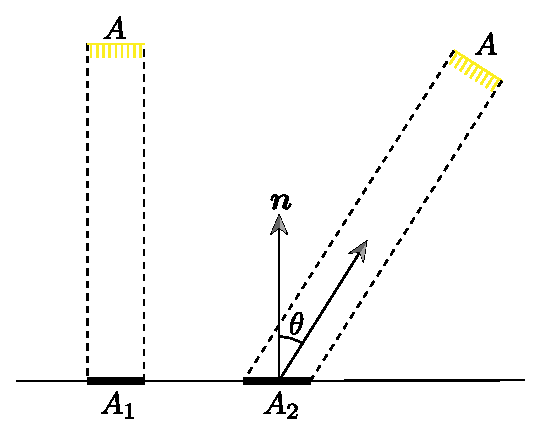
\includegraphics[width=0.4\linewidth]{chap05/LambertsLaw.eps}
    \caption{朗伯定律。到达表面的辐射照度随着入射角的余弦变化,
        因为更大的入射角有更大的照射区域。}
    \label{fig:5.7}
\end{figure}

\subsubsection*{立体角与强度}
为了定义强度,我们首先需要定义\keyindex{立体角}{solid angle}{}的表示
\sidenote{译者注:可参考译者补充的\refsub{辐射度量}。}。
立体角是平面上2D角拓展到球上的角。
\keyindex{平面角}{planar angle}{}是关于某位置朝向某物体的总角度(\reffig{5.8})。
考虑绕点$\bm p$的单位圆;如果我们将阴影物体投影到该圆上,该投影将覆盖一定长度的圆$s$。
$s$的弧长(等于角度$\theta$)即朝向物体的角度。
平面角单位为\keyindex{弧度}{radian}{}
\sidenote{译者注:一般简写为{\normalfont rad}。注意它是无量纲的导出单位。}。
\begin{figure}[htbp]
    \centering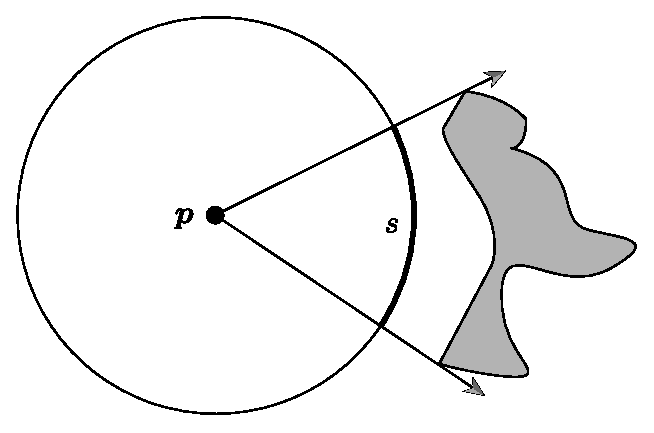
\includegraphics[width=0.5\linewidth]{chap05/Planarangle.eps}
    \caption{平面角。从点$\bm p$看物体的平面角等于从点$\bm p$朝它看所对的角度,
        或者等价地,单位圆上弧$s$的长度。}
    \label{fig:5.8}
\end{figure}

立体角把2D单位圆扩展到3D单位球(\reffig{5.9})。
总面积$s$即物体所对的立体角
\sidenote{译者注:更确切地说是面积与半径平方的比值。}。
立体角的单位为\keyindex{球面度}{steradian}{}(sr)
\sidenote{译者注:注意球面度也是无量纲的导出单位。}。
整个球体所对的立体角为$4\pi \text{sr}$,
半球对应$2\pi \text{sr}$。
\begin{figure}[htbp]
    \centering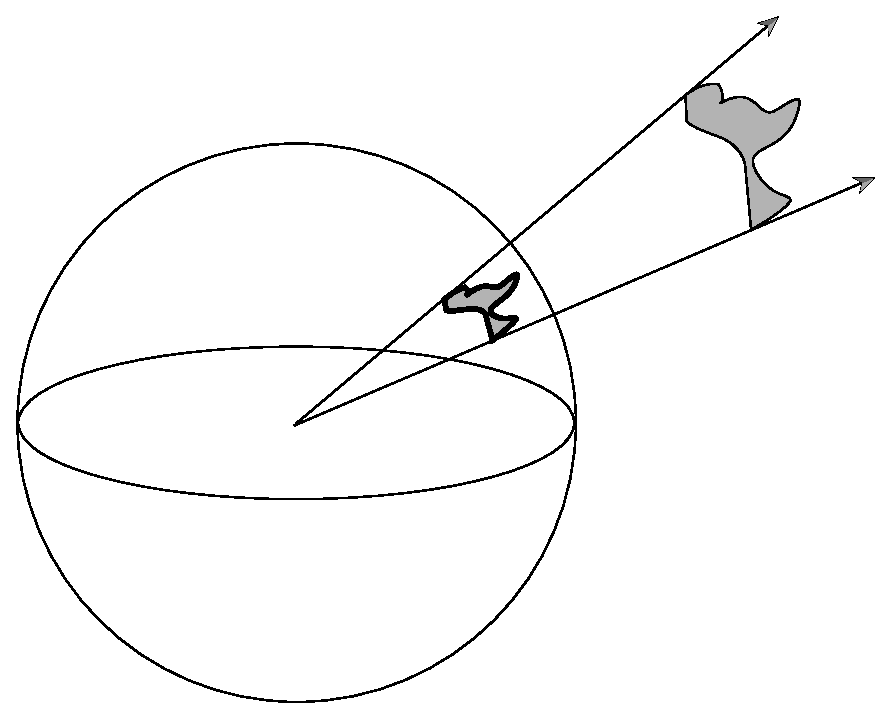
\includegraphics[width=0.5\linewidth]{chap05/Solidangle.eps}
    \caption{三维内物体$c$所对的立体角$s$通过将$c$投影到
        单位球上并度量其投影面积算得。}
    \label{fig:5.9}
\end{figure}

以$\bm p$为球心的单位球上的点集可以用来描述从$\bm p$发出的向量。
我们将经常使用符号$\bm\omega$来表示这些方向,
并且我们将约定$\bm\omega$是标准化的向量。

现在考虑无穷小光源发射光子。如果我们将该光源置于单位球球心处,
则我们可以计算出射功率的角密度。
表示为$I$的\keyindex{辐射强度}{radiant intensity}{}
\sidenote{译者注:原文写作intensity。}
就是这样的量;它的单位为$\text{W}/\text{sr}$。在整个球的方向上,我们有
\begin{align*}
    I=\frac{\varPhi}{4\pi}\, ,
\end{align*}
但更一般地我们感兴趣的是取微分方向锥的极限
\sidenote{译者注:这里原作者借用了记号$\bm\omega$,
    在该式以及后续几个式子中,它表示立体角大小,本质是个标量。
    有时它又表示方向,是个向量。读者应结合语境区分。}:
\begin{align*}
    I=\lim\limits_{\Delta{\bm\omega}\rightarrow 0}{\frac{\Delta\varPhi}{\Delta{\bm\omega}}}=\frac{\mathrm{d}\varPhi}{\mathrm{d}{\bm\omega}}\, .
\end{align*}

和平常一样,我们可以对强度积分回到功率:设强度是方向的函数$I({\bm\omega})$,
我们可以在有限方向集$\Omega$上积分以反求功率:
\begin{align*}
    \varPhi=\int\limits_{\Omega}I({\bm\omega})\mathrm{d}{\bm\omega}\, .
\end{align*}

强度描述了光的方向分布,但它只对点光源有意义。

\subsubsection*{辐射亮度}
最后,最重要的辐射度量数量是\keyindex{辐射亮度}{radiance}{}
\sidenote{译者注:也称辐亮度、辐射度。}$L$。
辐射照度和辐射出射度为我们给出了在点$\bm p$处
每块微分面积上的微分功率,但它们不区分功率的方向分布。
辐射亮度执行最后一步并度量关于立体角的辐射照度或辐射出射度。
它定义为
\begin{align*}
    L({\bm p},{\bm\omega})=\lim\limits_{\Delta{\bm\omega}\rightarrow 0}{\frac{\Delta E_{\bm\omega}({\bm p})}{\Delta{\bm\omega}}}=\frac{\mathrm{d}E_{\bm\omega}({\bm p})}{\mathrm{d}{\bm\omega}}\, ,
\end{align*}
其中我们已经用$ E_{\bm\omega}$表示垂直于方向$\bm\omega$的曲面上的辐射照度。
换句话说,辐射亮度并不是根据入射到$\bm p$所在表面上的辐射照度来度量的。
实际上,面积计算的这一变化利于抵消辐射亮度定义中来自朗伯定律的项$\cos\theta$。

辐射亮度是单位面积单位立体角上的通量密度。用通量表示时,它定义为
\begin{align}\label{eq:5.2}
    L=\frac{\mathrm{d}\varPhi}{\mathrm{d}{\bm\omega}\mathrm{d}A^{\perp}}\, ,
\end{align}
其中$\mathrm{d}A^{\perp}$是$\mathrm{d}A$在
垂直于$\bm\omega$的假想面上的投影面积(\reffig{5.10})。
因此,它是当所关心的入射方向锥$\mathrm{d}{\bm\omega}$变得非常小且
曲面上关心的局部面积$\mathrm{d}A$也变得非常小时对入射光度量的极限
\sidenote{译者注:该式分子的写法并不规范,但不影响理解,见\refeq{5.ex-radiance}。}。
\begin{figure}[htbp]
    \centering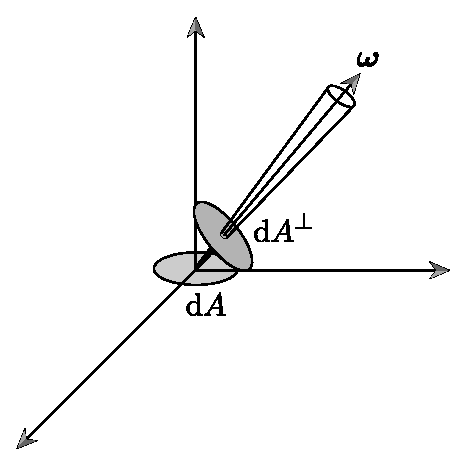
\includegraphics[width=0.4\linewidth]{chap05/Radiance.eps}
    \caption{辐射亮度$L$定义为单位立体角$\mathrm{d}{\bm\omega}$
    单位投影面积$\mathrm{d}A^{\perp}$上的通量。}
    \label{fig:5.10}
\end{figure}

所有这些辐射度量数量中,辐射亮度是贯穿本书剩余部分最频繁使用的量。
一个直观原因是在一些场景中它是所有辐射度量数量中最为基本的;
如果给定辐射亮度,则所有其他值都能通过在面积和方向上对辐射亮度积分而计算出来。
辐射亮度另一很好的性质是它在沿穿过空的空间的光线时保持不变。
因此它自然是光线追踪要计算的量。

\subsection{入射与出射辐亮度函数}\label{sub:入射与出射辐亮度函数}
当光线与场景中的曲面相交时,辐亮度函数$L$一般在曲面边界处不连续。
在完全不透明曲面(例如镜子)的极端情况下,辐亮度函数
在稍微高于和稍微低于曲面处的值可能完全无关。

因此在不连续处取单侧极限来区分上下方的辐亮度函数是有意义的
\sidenote{译者注:这里的$\bm\omega$是辐射传播方向,注意与下文区分。}:
\begin{align}\label{eq:5.3}
    L^+({\bm p},{\bm\omega}) & =\lim\limits_{t\rightarrow 0^+}{L({\bm p}+t{\bm n}_{\bm p},{\bm\omega})}\, ,\nonumber \\
    L^-({\bm p},{\bm\omega}) & =\lim\limits_{t\rightarrow 0^-}{L({\bm p}+t{\bm n}_{\bm p},{\bm\omega})}\, ,
\end{align}
其中${\bm n}_{\bm p}$是在$\bm p$处的曲面法线。
然而,全文保持跟踪单侧极限是自找麻烦。

我们更喜欢通过区分到达一点的辐亮度(例如取决于来自光源的照射)和
离开该点的辐亮度(例如取决于来自表面的反射)来解决歧义性。

考虑物体表面上的一点$\bm p$。
到达该点的辐亮度分布函数可由关于位置和方向的函数进行数学描述。
该函数记为$L_{\mathrm{i}}({\bm p},{\bm\omega})$(\reffig{5.11})。
描述该点从表面射出的反射辐亮度的函数记为$L_{\mathrm{o}}({\bm p},{\bm\omega})$。
注意两种情况下方向向量$\bm\omega$都指向远离$\bm p$的方向,
但要意识到一些作者为$L_{\mathrm{i}}$用的记号$\bm\omega$是翻转了的所以指向了$\bm p$。
\begin{figure}[htbp]
    \centering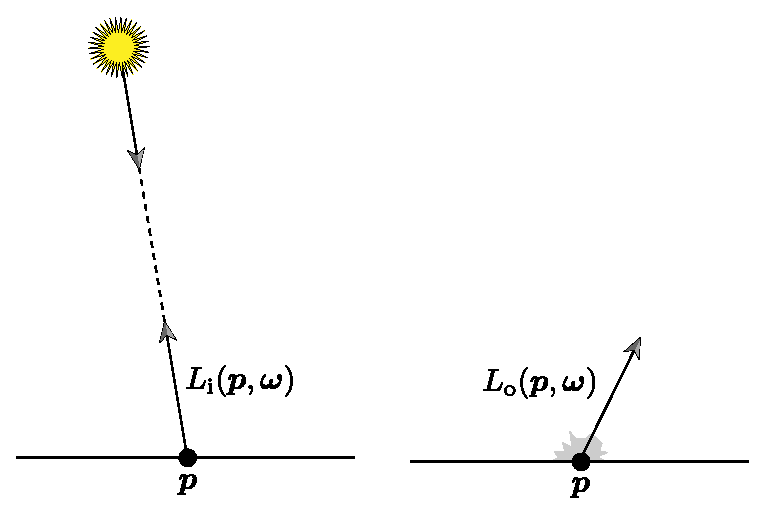
\includegraphics[width=0.6\linewidth]{chap05/Incidentoutgoingradiance.eps}
    \caption{(a)入射辐亮度函数$L_{\mathrm{i}}({\bm p},{\bm\omega})$把
    到达一点的辐亮度分布描述为位置和方向的函数。
    (b)出射辐亮度函数$L_{\mathrm{o}}({\bm p},{\bm\omega})$给出了离开该点的辐亮度分布。
    注意两个函数中$\bm\omega$都指向远离曲面的方向,
    进而例如$L_{\mathrm{i}}({\bm p},-{\bm\omega})$给出了
    到达$\bm\omega$所不在的曲面另一侧的辐亮度。}
    \label{fig:5.11}
\end{figure}

这些更直观的入射和出射辐亮度函数
与来自\refeq{5.3}的单侧极限之间有简单的联系:
\begin{align*}
    L_{\mathrm{i}}({\bm p},{\bm\omega}) & =\left\{
    \begin{array}{lr}
        L^+({\bm p},-{\bm\omega}), & {\bm\omega}\cdot{\bm n}_{\bm p}>0 \\
        L^-({\bm p},-{\bm\omega}), & {\bm\omega}\cdot{\bm n}_{\bm p}<0
    \end{array}
    \right.                                        \\
    L_{\mathrm{o}}({\bm p},{\bm\omega}) & =\left\{
    \begin{array}{lr}
        L^+({\bm p},{\bm\omega}), & {\bm\omega}\cdot{\bm n}_{\bm p}>0 \\
        L^-({\bm p},{\bm\omega}), & {\bm\omega}\cdot{\bm n}_{\bm p}<0
    \end{array}
    \right.
\end{align*}

全书中,我们将用入射和出射辐亮度函数的思想来解决边界处辐亮度函数的歧义性。

另一需要记住的性质是空间中没有曲面处的一点(即在自由空间中),
$L$是连续的,所以$L^+=L^-$,即意味着:
\begin{align*}
    L_{\mathrm{o}}({\bm p},{\bm\omega})=L_{\mathrm{i}}({\bm p},-{\bm\omega})=L({\bm p},{\bm\omega})\, .
\end{align*}
换句话说,$L_{\mathrm{i}}$和$L_{\mathrm{o}}$只有翻转的方向不同。

\subsection{光亮度与光度学}\label{sub:光亮度与光度学}
像辐通量、辐亮度等所有辐射度量都有对应的光度学度量。
\keyindex{光度学}{photometry}{}是依据人类视觉系统的感知针对可见电磁辐射的研究。
每个频谱辐射度量数量都能通过与描述人眼对不同波长相对敏感度的光谱响应曲线
$V(\lambda)$的积分转化为相应的光度学数量
\footnote{光谱响应曲线模型基于室内规范化照明环境下完成的实验。
    因为在暗环境下对颜色的敏感度会下降,所以它不能很好地对人类视觉系统在所有光照条件下的响应进行建模。
    然而,它构建了光亮度定义以及其他相关光度学性质的基础。}。

\keyindex{光亮度}{luminance}{}\sidenote{译者注:可简称亮度。}度量了
光谱功率分布对于人类观察者看起来有多亮。
例如,光亮度考虑了对于人类而言在绿色波段具有特定能量值的SPD会比
在蓝色区具有相同能量值的SPD看起来更亮这一事实。

我们将用$Y$表示光亮度;它与频谱辐亮度$L(\lambda)$的关系为
\begin{align*}
    Y=\int\limits_{\lambda}{L(\lambda)V(\lambda)\mathrm{d}\lambda}\, .
\end{align*}

光亮度和光谱响应曲线$V(\lambda)$与颜色的XYZ表示(\refsub{XYZ颜色})紧密相关。
CIE的$Y(\lambda)$三刺激曲线选为与$Y(\lambda)$成正比使得
\begin{align*}
    Y=683\int\limits_{\lambda}{L(\lambda)V(\lambda)\mathrm{d}\lambda}\, .
\end{align*}
光亮度的单位是坎德拉$/$米$^2$($\text{cd}/\text{m}^2$),
其中\keyindex{坎德拉}{candela}{}(cd)是辐射强度的光度学等价。
\reftab{5.1}给出了一些代表性的光亮度值。
\begin{table}[htbp]
    \centering
    \begin{tabular}{l c}
        \toprule
        \textbf{条件}    & \textbf{光亮度($\text{cd}/\text{m}^2$,旧称\keyindex{尼特}{nit}{})} \\
        \midrule
        地平线的太阳     & 600,000                                                               \\
        60瓦的灯泡       & 120,000                                                               \\
        晴朗的天空       & 8,000                                                                 \\
        典型办公室       & 100-1,000                                                             \\
        典型计算机显示器 & 1-100                                                                 \\
        街道照明         & 1-10                                                                  \\
        阴天月光         & 0.25                                                                  \\
        \bottomrule
    \end{tabular}
    \caption{多种光照条件下的代表性光亮度值。}
    \label{tab:5.1}
\end{table}

本章介绍的其他所有辐射度量数量均有光度学等价;
它们总结于\reftab{5.2}中
\footnote{各种光度学量有很不寻常的名字;Jim Kajiya很好地
    总结了这些令人有点容易搞晕的情况:“一尼特是每球面度上的一勒克斯,
    是每平方米上的一坎德拉,是每平方米每球面度上的一流明。明白了吗?”}
\sidenote{译者注:原书表中将焦耳的缩写误写为Q,已修正。}。
\begin{table}[htbp]
    \centering
    \begin{tabular}{llll}
        \toprule
        \textbf{辐射度量} & \textbf{单位}        & \textbf{光度学}                           & \textbf{单位}                           \\
        \midrule
        辐射能            & 焦耳(J)              & \keyindex{光能}{luminous energy}{}        & \keyindex{塔尔波特}{talbot}{}(塔,T)    \\
        辐射通量          & 瓦特(W)              & \keyindex{光通量}{luminous flux}{}        & \keyindex{流明}{lumen}{}(lm)            \\
        辐射强度          & W$/$sr               & \keyindex{发光强度}{luminous intensity}{} & lm$/$sr=坎德拉(cd)                      \\
        辐射照度          & W$/$m$^2$            & \keyindex{光照度}{illuminance}{}          & lm$/$m$^2$=\keyindex{勒克斯}{lux}{}(lx) \\
        辐射亮度          & W$/$(sr$\cdot$m$^2$) & 光亮度                                    & lm$/$(sr$\cdot$m$^2$)=cd$/$m$^2$=nit    \\
        \bottomrule
    \end{tabular}
    \caption{辐射度量及其光度学同型。}
    \label{tab:5.2}
\end{table}